\documentclass[main]{subfiles}
\begin{document}

\section*{Lecture 7 // Sept 15 // Outline of proof of Donaldson's theorem}
\addcontentsline{toc}{section}{Lecture 7 -- Outline of proof of Donaldson's theorem}

\begin{recall}
Let $(M^4,g)$ be positive definite and simply connected. Fix a $k=1$ $\SU(2)$ bundle $E$ over $M$. Set
\[
\mc{M} := \{\text{SD YM connections on } E\}/\mc{G}.
\]
Each splitting $L\oplus\bar L$ of $E$ has a unique (up to $\SU(2)$ gauge equivalence) split SDYM connection $\nabla\oplus\bar\nabla$ for which $F_\nabla$ is the unique harmonic representative of $c_1(L)$.

Today, we'll outline a proof of Donaldson's theorem by establishing qualitative features about $\mc{M}$.
\end{recall}

\begin{theorem*}[Donaldson (\cref{thm:donaldson})]
If $X^4$ is $\pi_1=1$, smooth, closed 4-manifold and $Q_X$ is definite, then $Q_X$ is equivalent to $n(+1)$ or $n(-1)$.
\end{theorem*}

\begin{claim}
\leavevmode
\begin{enumerate}
	\item Away from a finite number of singular points, $\mc{M}$ is a smooth 5-dimensional oriented manifold.
	\item The number of these points $=$ the \# of splittings of $E$.
	\item Each point has a neighborhood homeomorphic to cone on $\CC\mathrm{P}^2$; diffeomorphic away from point.
	\item $\mc{M}$ is \underline{not} compact, but it admits a compactification $\bar{\mc{M}}$ such that $\partial\bar{\mc{M}} \cong M$.
\end{enumerate}
\end{claim}

\begin{figure}[h]
\centering
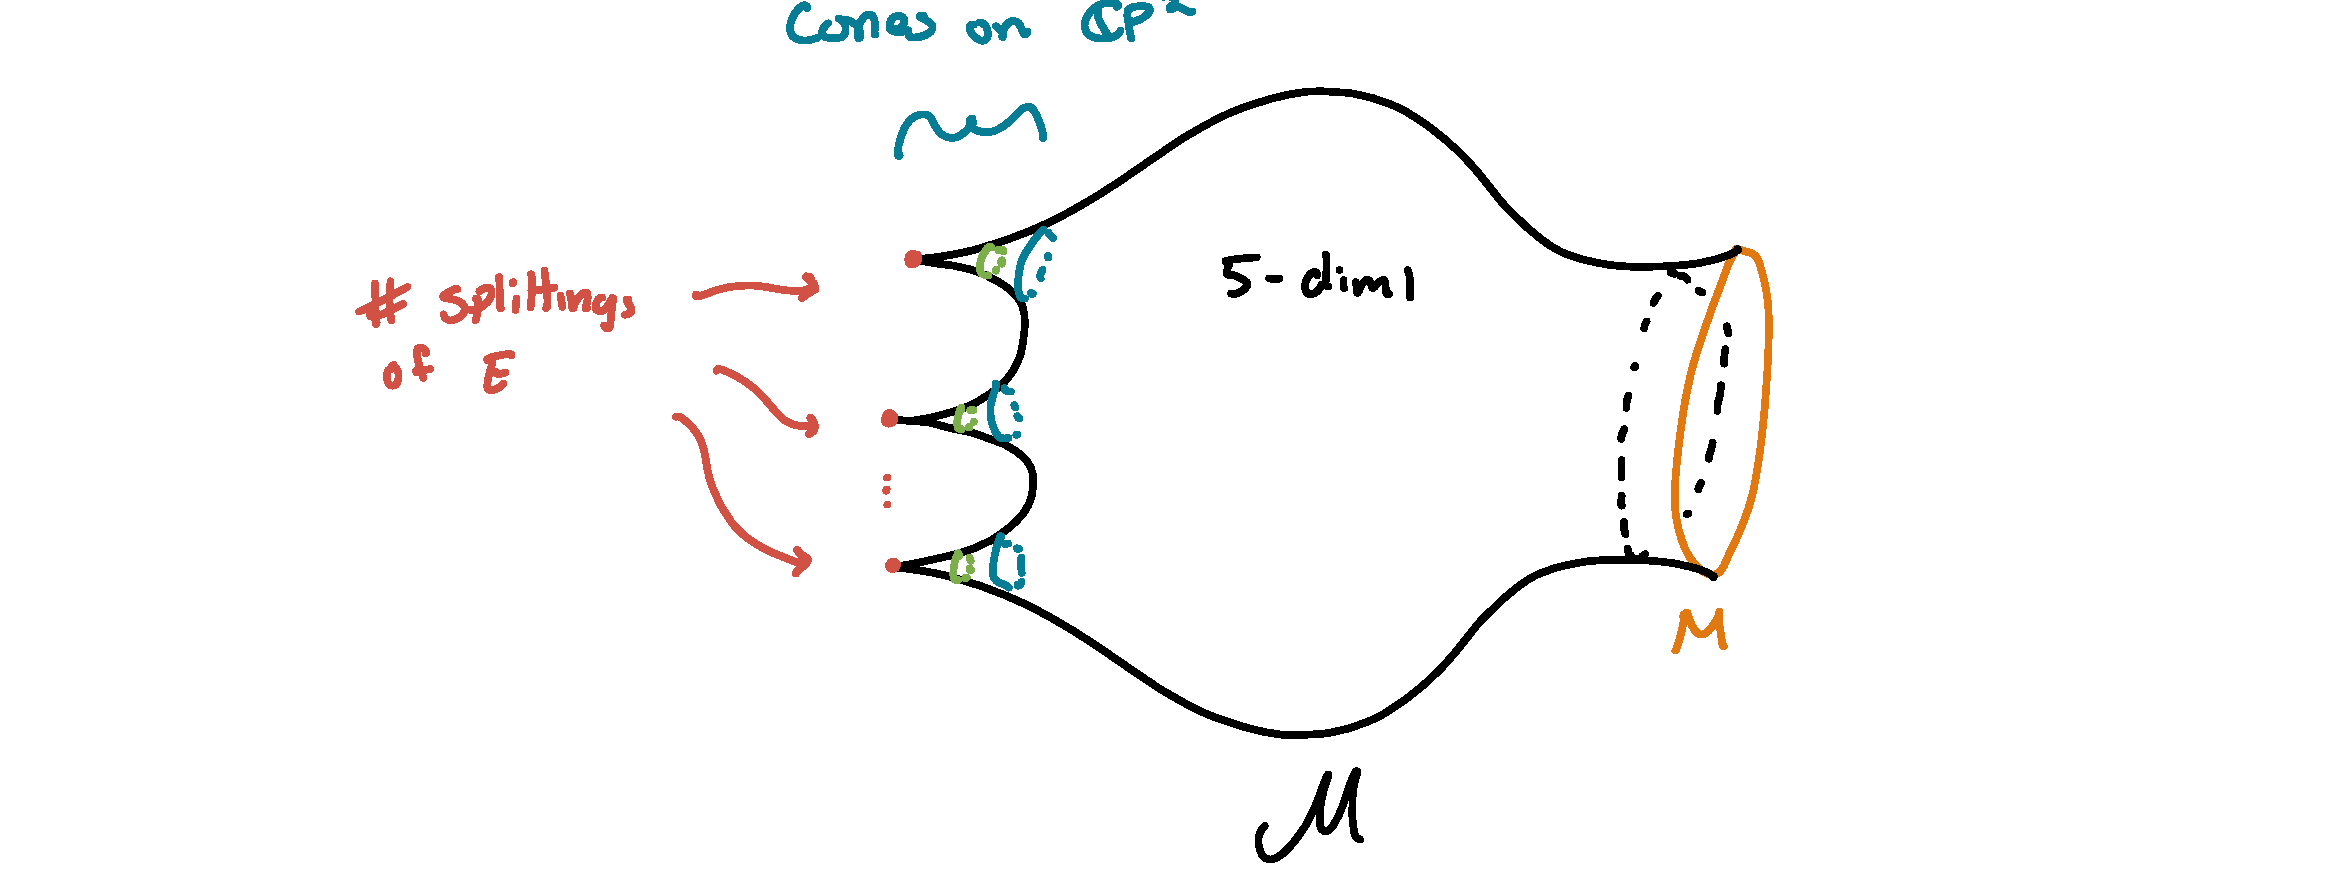
\includegraphics[width=0.85\textwidth]{figures/fig_lec7_moduli.png}
\end{figure}

\begin{wrapfigure}{r}{0.3\textwidth}
\centering
\vspace{-1em}
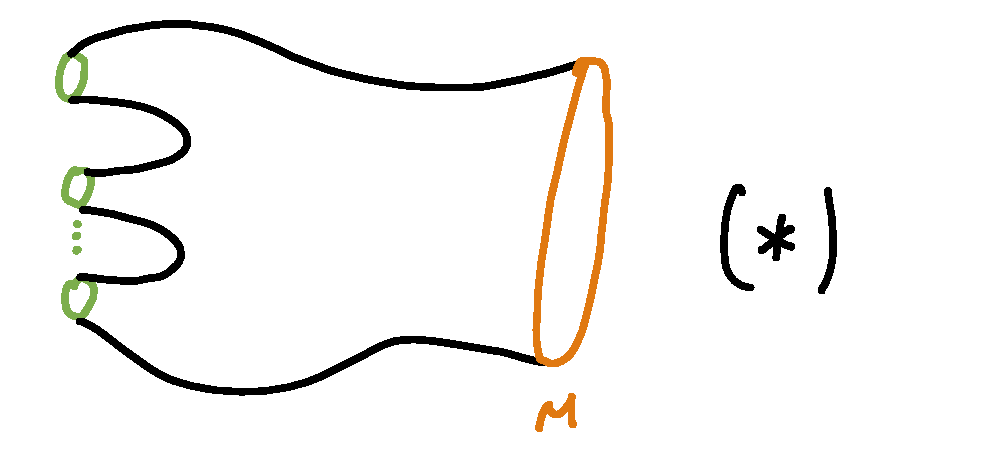
\includegraphics[width=\linewidth]{figures/fig_lec7_cobordism_star.png}
\end{wrapfigure}
We have a cobordism $M$ to $\bigsqcup_{\substack{\text{\#splittings}\\ \text{of } E}} \CC\mathrm{P}^2$ obtained by removing the singular points. \hfill $(\ast)$

It turns out that $(\ast)$ implies Donaldson's theorem. Before we discuss this, we'll briefly motivate why bordism is useful here.

\subsection*{Interlude: Bordism in General}

This discussion isn't strictly necessary, but it places $(\ast)$ in context.

\begin{definition}
\begin{minipage}[t]{0.62\textwidth}
The $n$-th bordism group is
\[
\Omega^n = \left\{\text{Set of all oriented smooth } n\text{-mfd.}\right\}/\sim
\]
where $Y_1 \sim Y_2$ iff there exists $W^{n+1}$ such that $\partial W = -Y_1 \sqcup Y_2$. If $Y_1 \sim Y_2$, they are called bordant. $\Omega^n$ is a group under disjoint union and/or connect sum.
\end{minipage}%
\hfill
\begin{minipage}[t]{0.33\textwidth}
\centering
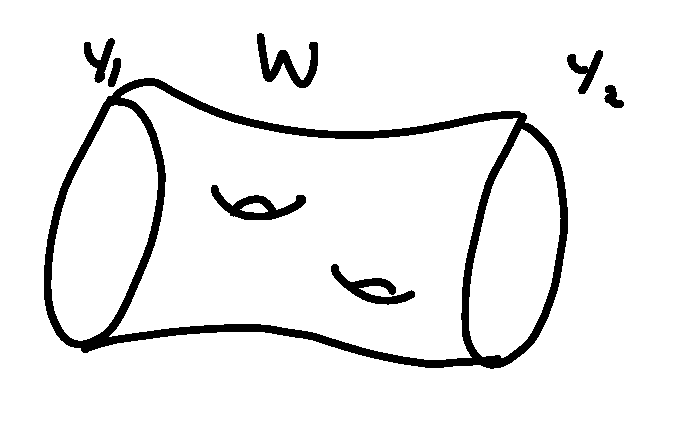
\includegraphics[width=\linewidth]{figures/fig_lec7_bordism_cylinder.png}\\[1em]
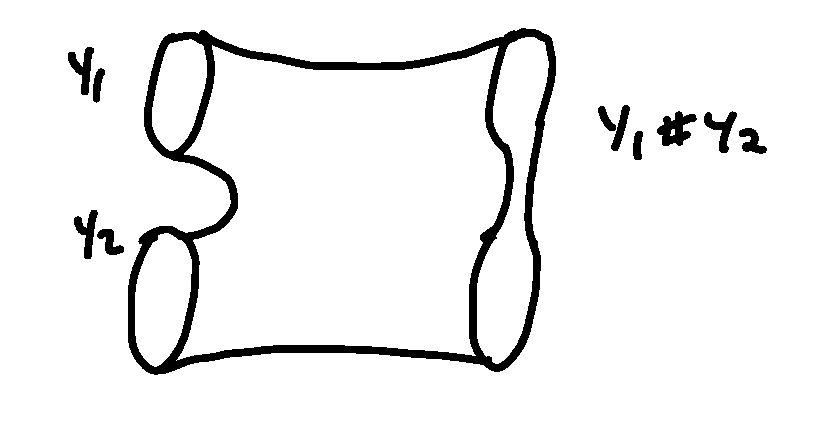
\includegraphics[width=\linewidth]{figures/fig_lec7_connect_sum.png}
\end{minipage}
\end{definition}

This is a generalization of the question: is $M^n \cong \partial W^{n+1}$ for some $W^{n+1}$? It turns out that in one of the great algebraic topology triumphs of the 60's, the groups $\Omega^n$ are well understood. In particular, $\Omega^n/\text{torsion}$ is known for all $n\in\NN$. Concretely, for $n=3$, $\Omega^3=0$ since every 3-manifold bounds a 4-manifold. When $n=4$, $\Omega^4 \cong \ZZ$, which is determined by signature.

\begin{definition}
The signature of a 4-manifold is $\sigma(M) = \sigma(Q_M) = \#\text{+eigenvalues} - \#\text{-eigenvalues}$.
\end{definition}

\begin{theorem}
In dimension 4, signature is a complete bordism invariant.
\end{theorem}

This means that two 4-manifolds are cobordant if and only if they have the same signature. In particular, any $M$ is cobordant to either $\#_{\sigma(M)} \CC\mathrm{P}^2$, if $\sigma(M)\geq 0$, or $\#_{-\sigma(M)} \overline{\CC\mathrm{P}^2}$, if $\sigma(M)<0$.

For our purposes, we'll only need the claim that $\sigma$ is a bordism invariant.

\begin{proposition}\label{prop:bordant-signature}
If $M_1$ and $M_2$ are bordant, then $\sigma(M_1) = \sigma(M_2)$.
\end{proposition}

To prove this proposition, we'll need the following lemma, commonly referred to as the ``half lives, half dies'' theorem.

\begin{wrapfigure}{l}{0.33\textwidth}
\centering
\vspace{-1em}
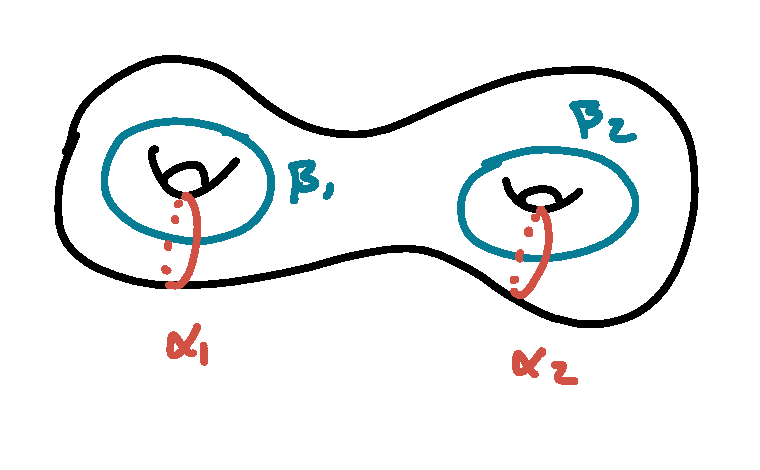
\includegraphics[width=\linewidth]{figures/fig_lec7_genus2.png}
\end{wrapfigure}
To motivate it, consider $Z_g = \partial H_g$. Think of $Z_g$ as a stand in for $M$ and $H_g$ a stand in for $W$. The middle dimension of the (co)homology of $Z$ is $H_1$, so we look at the map induced by the inclusion $\iota : Z_g \to H_g$.
\[
\iota_\ast : H_1(Z_g) \longrightarrow H_1(H_g)
\]
\[
\ker \iota_\ast \cong \operatorname{span}\{\alpha_1,\alpha_2\}
\]
\[
\operatorname{im} \iota_\ast \cong \operatorname{span}\{\iota_\ast(\beta_1), \iota_\ast(\beta_2)\}
\]

\begin{lemma}[Half lives, half dies]
For $W$ a smooth oriented $2n+1$ dimensional manifold with boundary $\partial W \cong M$, $\ker(\iota_\ast) \subset H_n(M;\RR)$ is a half-dimensional Lagrangian subspace with respect to the intersection form $Q : H^n(M;\RR)\times H^n(M;\RR) \to \ZZ$, where $\iota_\ast : H_n(M;\RR) \to H_n(W;\RR)$ is the map on homology induced by the inclusion $\iota : M \cong \partial W \hookrightarrow W$.
\end{lemma}

\begin{proof}[Proof of Lemma]
First recall that by Poincar\'e duality, $H_n(M;\RR) \cong H^n(M;\RR)$.

Further, from linear algebra, if $T : A \to B$ is a linear map, the dual map $T^\ast : B^\ast \to A^\ast$ is such that $\dim \operatorname{im} T = \dim \operatorname{im} T^\ast$:
\[
\dim \operatorname{im} T = \dim(A) - \dim(\ker T) = \dim(A/\ker T) = \dim(\operatorname{Ann}(\ker T)) = \dim \operatorname{im} T^\ast
\]
\[
\left(\operatorname{Ann}(\ker T) \text{ is the subspace of } A^\ast \text{ that annihilates } T\right)
\]

Thus the maps
\[
\iota^\ast : H^n(W;\RR) \longrightarrow H^n(M;\RR), \qquad \iota_\ast : H_n(M;\RR) \longrightarrow H_n(W;\RR)
\]
are dual in the linear algebra sense, so $\dim \operatorname{im} \iota^\ast = \dim \operatorname{im} \iota_\ast$.

Again by Poincar\'e duality, $\dim \operatorname{im} \iota^\ast = \dim \ker \iota_\ast$.

Thus
\[
\dim \ker \iota_\ast + \dim \operatorname{im} \iota_\ast = \dim H_n(M;\RR)
\]
\[
\dim \operatorname{im} \iota^\ast + \dim \operatorname{im} \iota^\ast
\]
\[
\Rightarrow \dim \operatorname{im} \iota^\ast = \tfrac12 \dim H_n(M;\RR) = \tfrac12 \dim H^n(M;\RR)
\]
\[
\Rightarrow \dim \ker \iota_\ast = \tfrac12 \dim H_n(M;\RR)
\]

Now, take $\alpha,\beta \in H^n(W;\RR)$, so $\iota^\ast(\alpha), \iota^\ast(\beta) \in H^n(M;\RR)$.

Then
\[
Q_M\big(\iota^\ast(\alpha), \iota^\ast(\beta)\big) = \int_M \iota^\ast(\alpha)\wedge\iota^\ast(\beta) = \int_M \iota^\ast(\alpha\wedge\beta) = \int_{\partial W} \iota_\ast(\alpha\wedge\beta)
\]

By Stokes' theorem,
\[
\int_{\partial W} \iota_\ast(\alpha\wedge\beta) = \int_W d(\alpha\wedge\beta) = 0.
\]

Thus $\operatorname{im}(\iota^\ast)$ is Lagrangian with respect to $Q_M$. \qedhere
\end{proof}

\begin{remark}
We may avoid using Stokes' theorem by translating to algebraic topology and cupping against the fundamental class. Thus half lives half dies is true when $M$ isn't smoothable.
\end{remark}

Having proven half lives half dies, we may now prove the original proposition.

\begin{proposition*}[\cref{prop:bordant-signature}]
If $M_1$ and $M_2$ are bordant, then $\sigma(M_1) = \sigma(M_2)$.
\end{proposition*}

\begin{proof}
\begin{enumerate}
	\item By setting $M = -M_1\#M_2$, we know that $M \cong \partial(W^5)$. So it is enough to show that $\sigma(M) = 0$.
	\item Consider the long exact sequence in homology and the Poincar\'e-Lefschetz isomorphism. By naturality, the following diagram commutes:
	\[
	\begin{tikzcd}[column sep=1.4em]
	\cdots \arrow[r] & H^2(W;\RR) \arrow[r, "\iota^\ast"] \arrow[d, "PD"', "\cong"] & H^2(M;\RR) \arrow[r] \arrow[d, "PD"', "\cong"] & H^3(W,M;\RR) \arrow[r] \arrow[d, "PD"', "\cong"] & \cdots \\
	\cdots \arrow[r] & H_3(W,M;\RR) \arrow[r] & H_2(M;\RR) \arrow[r, "\iota_\ast"] & H_2(W;\RR) \arrow[r] & \cdots
	\end{tikzcd}
	\]
	Note that $\operatorname{im}\iota^\ast \cong \ker\iota_\ast$ under PD.
	\item By Half lives, half dies,
	\[
	\begin{cases}
	\dim \operatorname{im} \iota^\ast = \tfrac12 \dim H^2(M;\RR) \\
	\dim \ker \iota_\ast = \tfrac12 \dim H_2(M;\RR)
	\end{cases}
	\]
	and $Q_M$ vanishes on $\operatorname{im}\iota^\ast$ (e.g., $\operatorname{im}\iota^\ast \subset H^2(M;\RR)$ is Lagrangian).

	Thus there is a half-dimensional subspace on which the intersection form vanishes.
	\item This implies $\sigma(M)=0$: consider the diagonalization of $Q_M$ over $\RR$: $Q_M \cong \begin{pmatrix}+I & 0 \\ 0 & -I\end{pmatrix}$.
	\[
	\begin{pmatrix}+I & 0 \\ 0 & -I\end{pmatrix} V = V_+ \oplus V_-
	\]
	This splits $V$ into $V_+\oplus V_-$, where $Q_M$ is $\pm$-definite on $V_\pm$.

	Let $a = \dim V_+$ and $b = \dim V_-$. Then $a+b = \dim V_+ + \dim V_- = \dim V = 2k$.

	Let $U = \operatorname{im}\iota^\ast$. Since $Q_M$ vanishes on $U$, $U\cap V_+ = \{0\}$ and $U\cap V_- = \{0\}$.

	Thus
	\[
	\dim(U+V_+) = \dim(U) + \dim(V_+) = k+a \leq 2k
	\]
	\[
	\dim(U+V_-) = \dim(U) + \dim(V_-) = k+b \leq 2k
	\]
	\[
	\Rightarrow a\leq k,\ b\leq k. \text{ Since } a+b=2k,\ a=b=k \Rightarrow \sigma(M) = a-b = 0. \qedhere
	\]
\end{enumerate}
\end{proof}

\subsection*{Back to Donaldson}

Let's return to Donaldson and take stock of what we know:

\begin{theorem*}[Donaldson (\cref{thm:donaldson})]
If $X^4$ is $\pi_1=1$, smooth, closed 4-manifold and $Q_X$ is definite, then $Q_X$ is equivalent to $n(+1)$ or $n(-1)$.
\end{theorem*}

The previous discussion of bordism has given us the following three facts, from which Donaldson's theorem will follow.

\begin{enumerate}
	\item[(i)] $\sigma(M) = \operatorname{rk}(Q_M)$ (since $M$ is positive definite).
	\item[(ii)] $\sigma(M) = \#$ splittings of $E$.

	Since
	\begin{enumerate}
		\item $\sigma$ bordism invariant (Interlude)
		\item $M$ bordant to $\displaystyle\bigsqcup_{\substack{\text{\#splittings}\\ \text{of } E}} \CC\mathrm{P}^2$ $(\ast)$
	\end{enumerate}
	\item[(iii)] $\#$ splittings of $E = \tfrac12 \# x \in H^2$ such that $\langle x,x\rangle = 1$.

	This follows from two claims about vector bundles over $X^4$:
	\begin{enumerate}
		\item $\SU(2)$ bundles are determined by $c_2 \in H^4$ (true only in our setting)
		\item $\mathrm{U}(1)$ bundles are determined by $c_1 \in H^2$ (true in general)
	\end{enumerate}
	Via the curvature form or by formal properties of Chern classes, to say $E = L\oplus\bar L$ implies that $c_2(E) = c_1(L)\cup c_1(\bar L) = -c_1(L)\cup c_1(L)$.

	Similarly, if $c_2(E) = -x^2$ for $x\in H^2$, the above calculation implies that $E = L\oplus\bar L$. Note here that different choices of $x$ give different $L$'s in the splitting.

	Therefore, if $k = c_2(E) = 1$, we must search over $x\in H^2$ for which $x^2=1$.
\end{enumerate}

Combining (i), (ii), and (iii), we can see that
\[
\sigma(M) = \operatorname{rk}(Q_M) = \#\text{splittings of } E = \tfrac12 \# x\in H^2 \text{ s.t.\ } x^2=1.
\]
Heuristically, this equality says that $Q_M$ has ``many'' $x$ with $\langle x,x\rangle=1$, where ``many'' is exactly twice the number of splittings.

To prove Donaldson's theorem, it remains to show that $Q_M$ is equivalent to $n(+1)$ or $n(-1)$, i.e., $\pm n = \operatorname{rk}(Q_M) = \tfrac12 \# x\in H^2$ such that $x^2=1$.

\begin{lemma}
Let $Q : V\times V \to \ZZ$ be a positive-definite symmetric unimodular bilinear pairing. Then $\# x$ such that $Q(x,x)=1 \leq 2\operatorname{rk} Q$, with equality iff $Q$ is equivalent to $I$ over $\ZZ$.
\end{lemma}

Assuming the lemma, since $\operatorname{rk}(Q_M) = \tfrac12 \# x\in H^2$ such that $x^2=1$, where $x^2$ is shorthand for $Q(x,x)$, we get that
\[
\#x \text{ s.t.\ } Q(x,x)=1 \leq 2\cdot\tfrac12 \#x\in H^2 \text{ s.t.\ } Q(x,x)=1
\]
\[
\#x \text{ s.t.\ } Q(x,x)=1 \leq \#x\in H^2 \text{ s.t.\ } Q(x,x)=1
\]
So clearly we must have equality, so the lemma implies that $Q$ is equivalent to $I$ over $\ZZ$, thus $Q \cong \pm(n)$. This proves Donaldson's theorem.

We now prove the lemma.

\begin{proof}[Proof of Lemma]
First note that if $Q=I$, there is clearly $2\cdot\operatorname{rk} Q$ of such elements of $H^2$, since the standard basis vectors $e_i$ have self pairing $1$, as well as $-e_i$.

For a general $Q$, we'll apply the Gram-Schmidt process over $\ZZ$. Let $x$ be such that $Q(x,x)=1$. We claim that $V = \langle x\rangle \oplus \langle x\rangle^\perp$. Indeed, since any $z\in V$ decomposes as
\[
z = \underbrace{Q(x,x)x}_{\in\langle x\rangle} + \underbrace{(z-Q(x,z)x)}_{\in\langle x\rangle^\perp}
\]
we know that $V = \langle x\rangle + \langle x\rangle^\perp$; since $\langle x\rangle \cap \langle x\rangle^\perp = \{0\}$, this decomposition is orthogonal.

Thus $Q : \langle x\rangle\oplus\langle x\rangle^\perp \times \langle x\rangle\oplus\langle x\rangle^\perp \to \ZZ$, so $Q$ splits as a block matrix
\[
Q = \left(\begin{array}{c|c} 1 & 0 \\ \hline 0 & \ast \end{array}\right)
\begin{array}{l} \left.\rule{0pt}{1.1em}\right\}\ \langle x\rangle \\ \left.\rule{0pt}{1.1em}\right\}\ \langle x\rangle^\perp \end{array}
\]

Now, notice the following:
\begin{enumerate}
	\item $Q$ is still positive definite on $x^\perp$.
	\item Any $z\in V$ such that $Q(z,z)=1$ is either $\pm x$ or lies entirely in $\langle x\rangle^\perp$: if $z = cx+w$ for $w\in x^\perp$, $Q(z,z) = c^2 + \langle w,w\rangle \neq 1$.
	\item The rank of $Q|_{\langle x\rangle^\perp}$ is $\operatorname{rank}(Q)-1$.
\end{enumerate}

Thus we may proceed by induction on $Q|_{\langle x\rangle^\perp} : \langle x\rangle^\perp \times \langle x\rangle^\perp \to \ZZ$. If $\langle x\rangle^\perp$ contains no elements for which $x^2=1$, the process concludes, and the number of elements for which $x^2=1$ is necessarily less than $2\cdot\operatorname{rk}(Q)$. Otherwise, $Q$ can be completely diagonalized, so $Q$ is equivalent to $I$. \qedhere
\end{proof}

\end{document}
